\documentclass[twoside,twocolumn]{article}
\usepackage[UTF8]{ctex}
\usepackage{graphicx}   % 插入图片
\usepackage{blindtext}  % 虚拟文字
\usepackage[sc]{mathpazo} % Use the Palatino font
\usepackage[T1]{fontenc} % Use 8-bit encoding that has 256 glyphs
\linespread{1.05} % Line spacing - Palatino needs more space between lines
\usepackage{microtype} % Slightly tweak font spacing for aesthetics

\usepackage[english]{babel} % Language hyphenation and typographical rules

\usepackage[hmarginratio=1:1,top=32mm,columnsep=20pt]{geometry} % Document margins
\usepackage[hang, small,labelfont=bf,up,textfont=it,up]{caption} % Custom captions under/above floats in tables or figures
\usepackage{booktabs} % Horizontal rules in tables
\renewcommand{\figurename}{图}
\usepackage{datetime} %日期
\renewcommand{\today}{\number\year 年 \number\month 月 \number\day 日}

\usepackage{lettrine} % 首字符放大
\usepackage[super,square]{natbib}   % 使用上标
\bibliographystyle{unsrt}           % 按引用顺序排序
\usepackage{enumitem} % Customized lists
\setlist[itemize]{noitemsep} % Make itemize lists more compact

\usepackage{abstract} % Allows abstract customization
\renewcommand{\abstractnamefont}{\normalfont\bfseries} % Set the "Abstract" text to bold
\renewcommand{\abstracttextfont}{\normalfont\small\itshape} % Set the abstract itself to small italic text

\usepackage{titlesec} % Allows customization of titles
\renewcommand\thesection{\Roman{section}} % Roman numerals for the sections
\renewcommand\thesubsection{\arabic{subsection}} % roman numerals for subsections
\titleformat{\section}[block]{\large\scshape\centering}{\thesection.}{1em}{} % Change the look of the section titles
\titleformat{\subsection}[block]{\large}{\thesubsection.}{1em}{} % Change the look of the section titles
% 页眉页脚设计
\usepackage{fancyhdr} % Headers and footers
\pagestyle{fancy} % All pages have headers and footers
\fancyhead{} % Blank out the default header
\fancyfoot{} % Blank out the default footer
\fancyhead[C]{矿场资源经济学结课报告} % Custom header text
\fancyfoot[RO,RE]{\thepage} %  页脚,RO,CO,LO,右对齐,居中,左对齐

\usepackage{titling} % Customizing the title section
\setlength{\droptitle}{-4\baselineskip} % Move the title up

\pretitle{\begin{center}\Huge\bfseries} % Article title formatting
\posttitle{\end{center}} % Article title closing formatting
\title{稀土的应用与发展趋势} % Article title
\author{
    \textsc{北巷的猫} \\% Your name
    \normalsize 班级:松鼠2020班 \qquad 学号:22222222222 \\ % Your institution
    \normalsize 排版引擎:\LaTeX{}% Your email address
}
\date{\today}       %  日期
\bibliographystyle{plain}
\renewcommand{\maketitlehookd}{%
\renewcommand{\abstractname}{摘\qquad要}
    \begin{abstract}
    \noindent

China is a major country,has a considerable advantage in rare earth reserves and production , the reserves of the world's first, the world's largest production, wide distribution of soil, north ShanDong province and Inner Mongolia, south Sichuan and seven southern provinces. In our country, the rare earth has very extensive application in the industry, metallurgy, oil chemical industry, glass got very good application, also be used as the materials of rare earth rare earth can be used as luminescent materials, permanent magnet materials, in the synthesis of polymer materials has also made great progress, especially in the aspect of permanent magnetic material, with the development of computer technology, the application of rare earth gradually shifted from traditional industries to high-tech fields. In the medical aspect has also obtained many research results.

In recent years, the world's demand for rare earth is also increasing day by day. Throughout the past decades, people's demand for rare earth has always shown a growing trend. People's exploration of rare earth has never stopped, and the application of rare earth has gradually penetrated into every aspect of people's life. With the application of rare earth in the field of high and new technology and the exploration in medical treatment, it can be seen that rare earth still has great potential to be explored. Therefore, the development prospect of rare earth in the future is bright.

    \end{abstract}
}
\begin{document}

% Print the title
\maketitle
%----------------------------------------------------------------------------------------
%	ARTICLE CONTENTS
%----------------------------------------------------------------------------------------

\section{稀土简介}
\lettrine[nindent=0em,lines=2]{稀}{土}
(Rare Earth),是化学周期表中镧系元素和钪、钇共十七种金属元素的总称。有着“工业维生素”的美称。稀土的应用范围广泛,在军事、工业、农业、医学方面都有着相当重要的用途,尤其是随着现代电子信息技术的发展,稀土的用途也逐渐向高新科技领域迈进。中国已经成为世界上唯一的可以大量供应不同品种及不同品级稀土产品的国家, 在世界稀土市场上具有支配和主导地位,并且有着完善的产业链,而且稀土是我国的战略资源,因此我们有必要研究稀土的经济价值与前景。

世界上含有稀土元素的矿物越有250多种,但是真正具有开采价值的稀土矿物仅有10多种,其中最主要的是氟碳铈矿、独居石和离子吸附型矿。世界上主要稀土储藏国有中国、俄罗斯、美国、澳大利亚和印度,已探明的储量中,中国为3600万吨,美国至少有1300万吨,俄罗斯1900万吨。\cite{RN6}\\
\begin{figure}[ht]
  \centering
  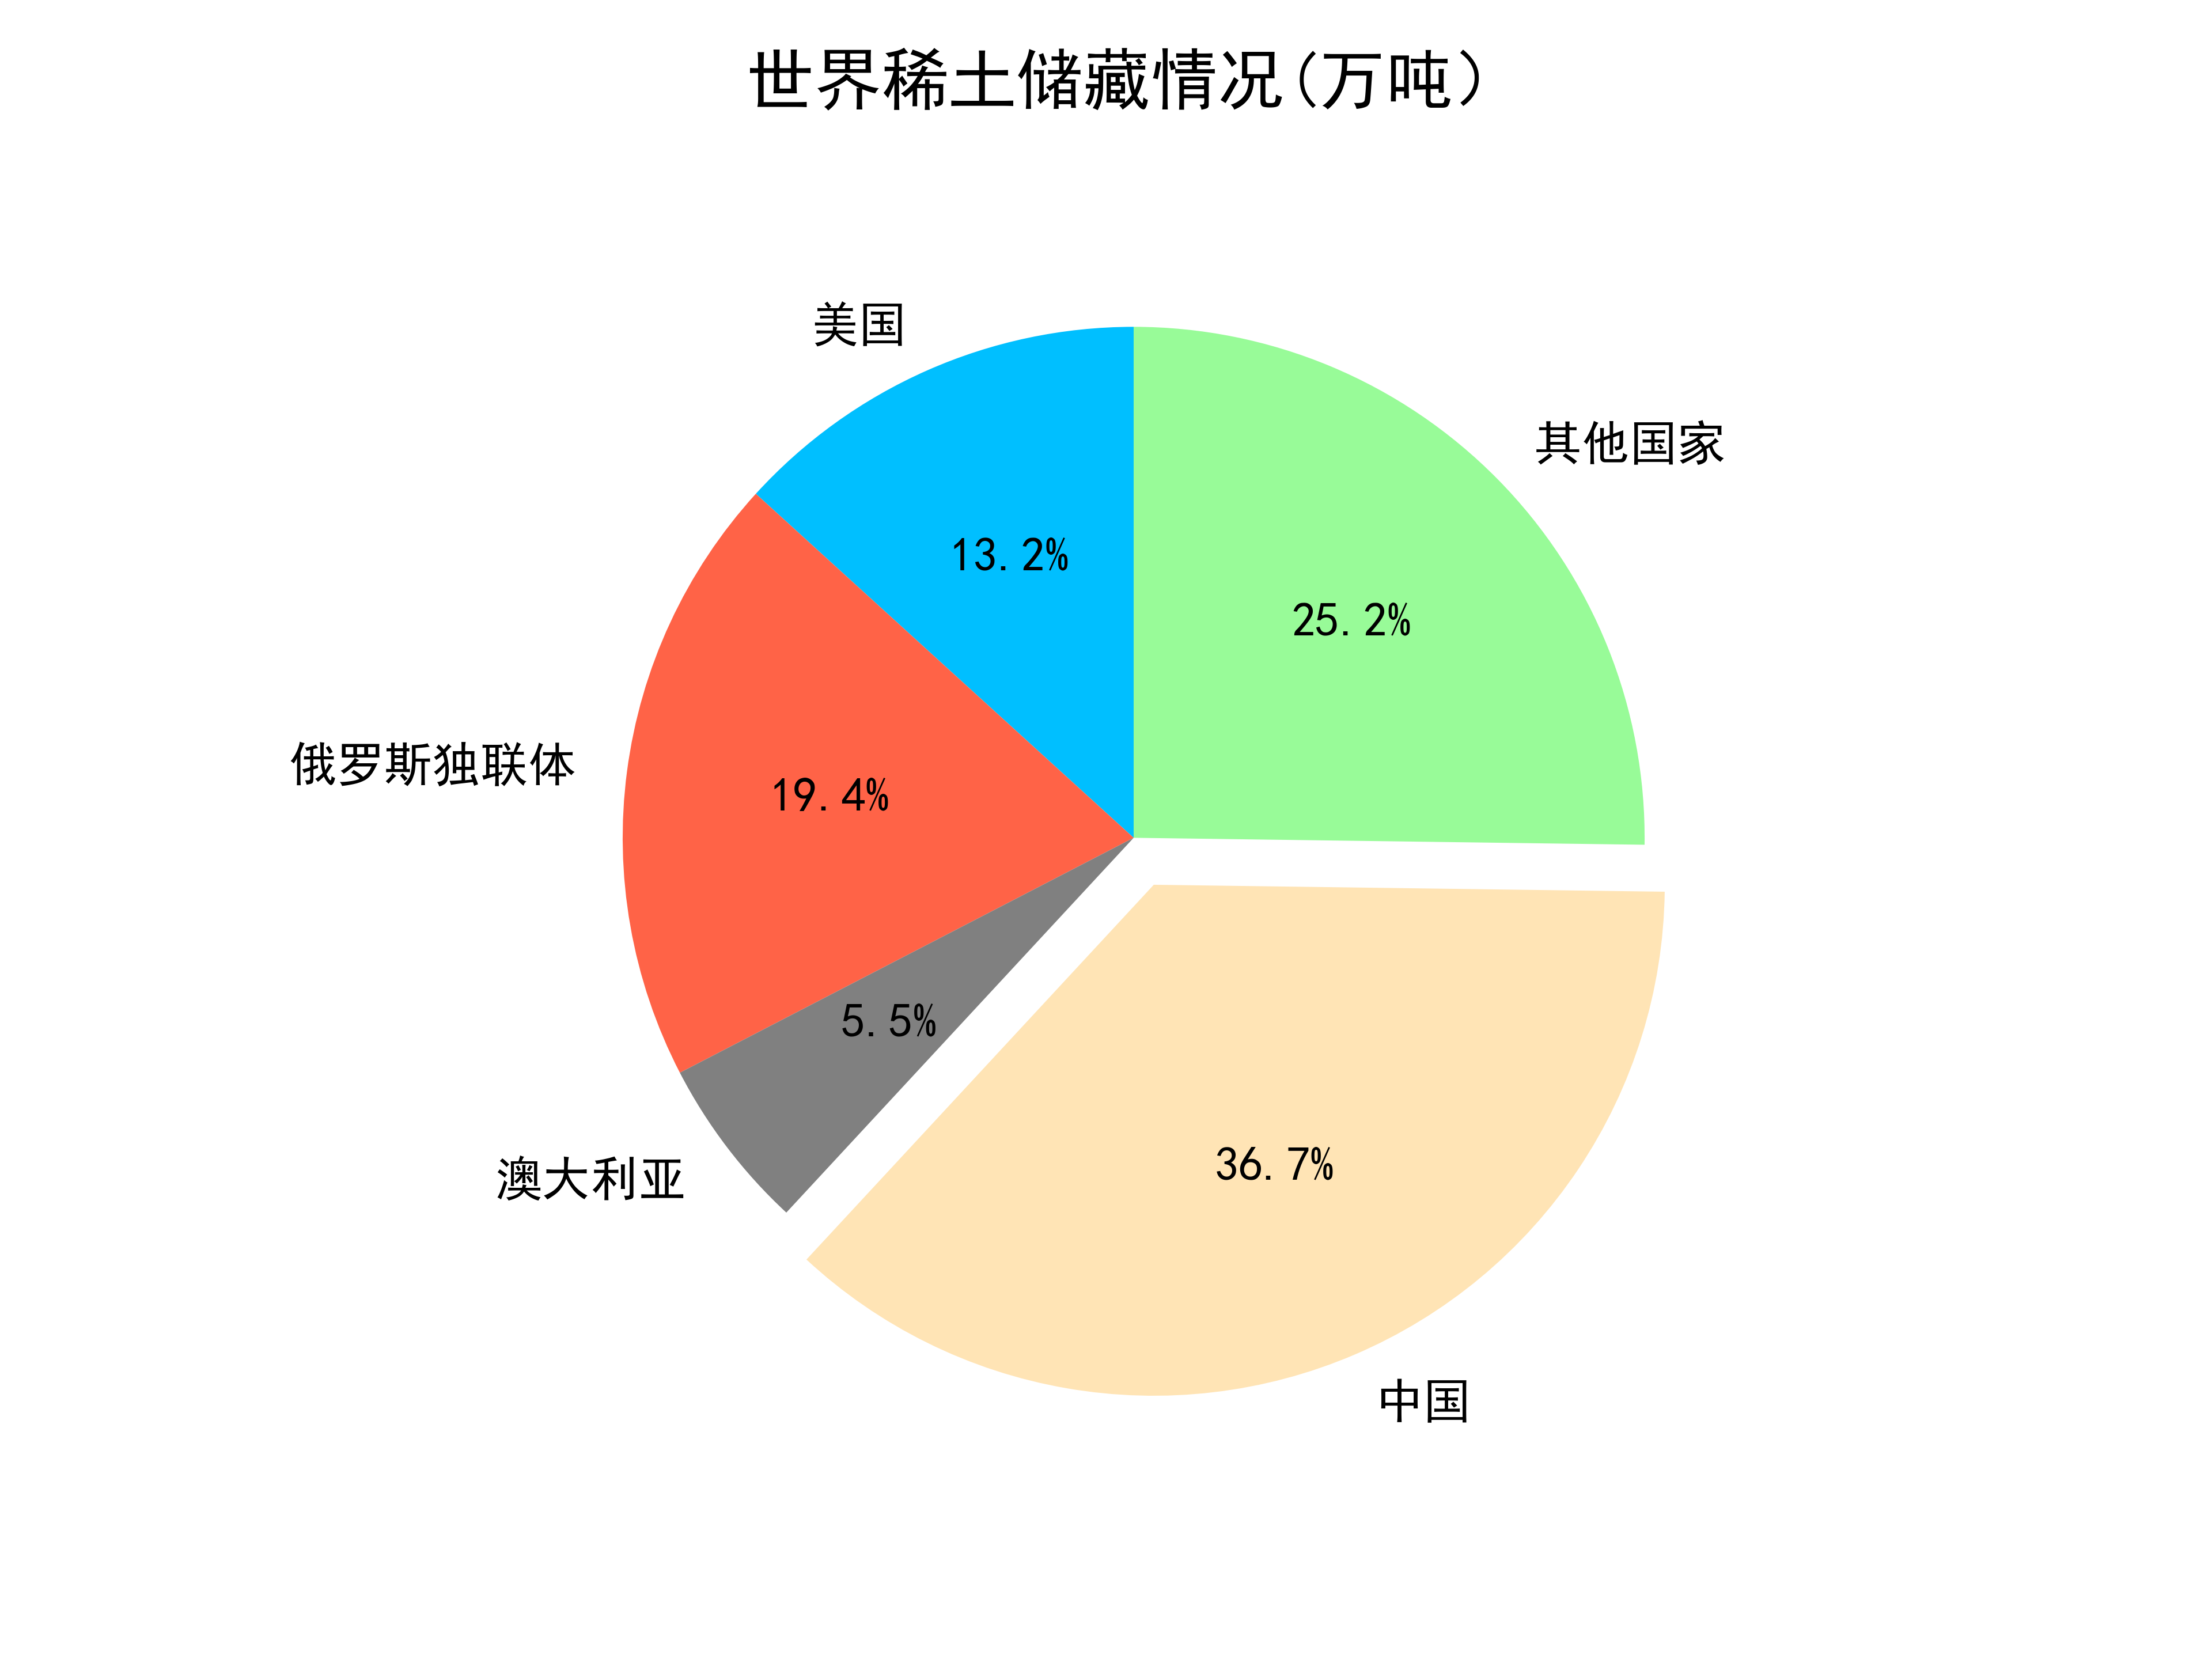
\includegraphics[width=22em]{figure4.png}
  \caption{世界稀土储藏情况\cite{RN6}}
\end{figure}

\begin{figure*}[ht]
  \centering
  \includegraphics{figure2.png}
  \caption{中国稀土矿床(点)分布图\cite{RN39}}
\end{figure*}

\section{我国稀土的分布和现状}

我国是世界稀土资源大国, 据1993 年1月美国矿物局出版的统计资料表明, 世界稀土工业储量为1 亿吨( REO ), 中国为430 万吨, 占世界总储量的43$\%$。我国稀土资源的特点是储量大、类型多、品种全、质量好、开采成本低,目前开发利用的稀土矿物主要有五种:氟碳铈矿、离子吸附型稀土矿、独居石矿、磷钇矿和磷灰石矿, 前四种矿占世界稀土产量的95 $\%$以上。除Pm 外的16 个稀土元素, 在我国从南到北分布齐全。中国稀土矿主要有白云鄂博矿, 四川冕宁矿, 山东微山矿, 南方七省的离子吸附型稀土矿, 广东、广西、江西的磷钇矿, 湖南、广东、广西、海南、台湾的独居石矿, 贵州含稀土的磷矿, 长江重庆段淤砂中的钪矿, 以及漫长海岸线上的海滨砂矿等。目前已形成了良好的生产布局, 产量稳居世界首位。\cite{RN6}
虽然我国的稀土资源居世界第一,但由于稀土应用水平较低等原因,我国稀土资源产业长期存在资源过度开采、大范围低价输出、不当开采引发环境污染难以处理等问题,资源优势没有相应产业化为经济优势。近些年来,稀土在整个国家发展中发挥了日益显著的作用,稀土问题越来越受到政府的高度重视,相继出台了一系列政策措施,在提高稀土出口价格、防治过度开采等方面取得了一定的进展。但稀土开采带来生态环境破坏以及滥采乱挖等问题仍然未能根治。

%------------------------------------------------

 \begin{figure}
  \centering
  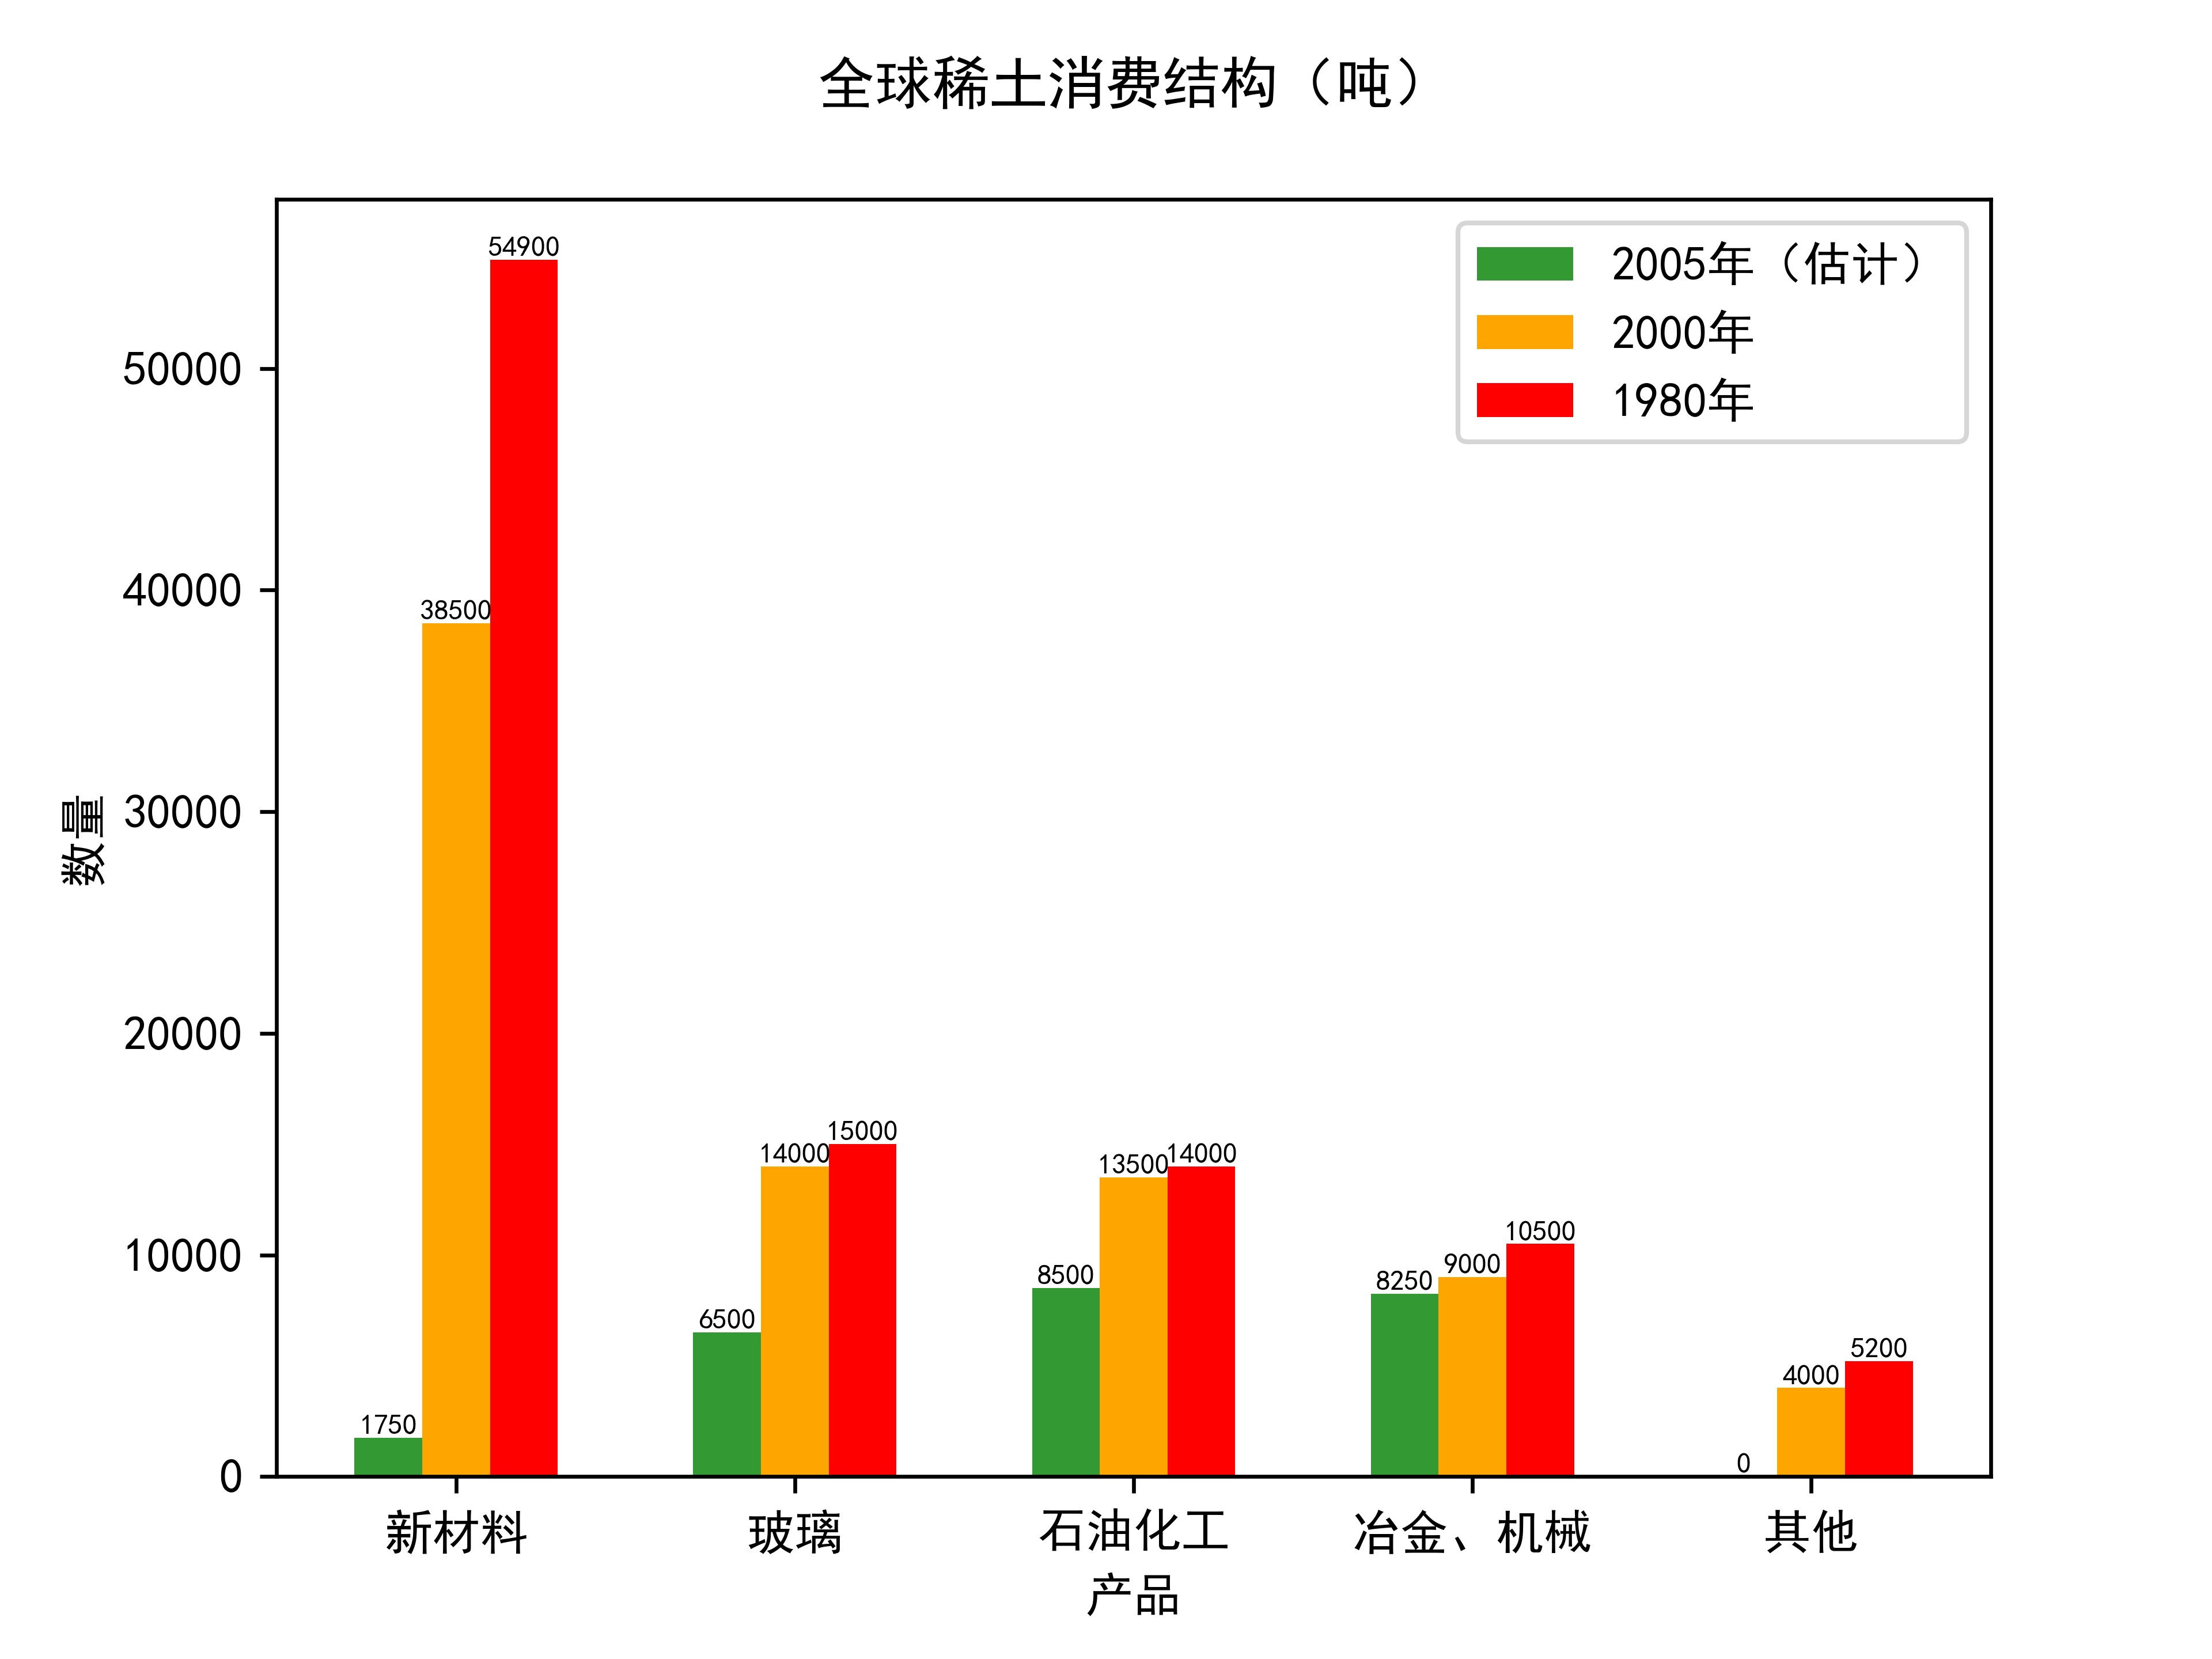
\includegraphics[width=20em]{figure6.png}
  \caption{全球稀土消费结构\cite{RN2}}
\end{figure}

\section{稀土的应用领域}
\subsection{冶金领域}
从1968年美国一家钢铁公司发现,在钢中加入稀土稀土,能大大改善钢的性能,提高了钢的冷变形能力,从而不易出现裂纹,这一成果不仅是得美国稀土在冶金领域的需求大幅增长,也为稀土开辟了一个新的应用领域,1981年直接增加到了历年的最高值6800吨(REO),但是20世纪70年代随着炼钢技术的发展,人们逐渐用更便宜的钙取代稀土,使得稀土在该领域的空间逐渐缩小,技术替代和材料替代使得20多年来,稀土在冶金、机械领域的消费徘徊不前。\cite{RN2}稀土在钢铁冶金中的应用是中国稀土的最大消费领域,特别是在铸铁中的应用很普遍,从1991年到1995年呈逐年增长的的趋势,在钢中的应用相应的小一些,而且需求逐年减少。稀土在铸铁中的作用主要是作为球化剂、蠕化剂和孕育剂使用,稀土在钢铁中的应用的绝对量在增加,但所占国内应用量比例却是在降低。\cite{RN55}

\begin{figure}[h]
   \centering
   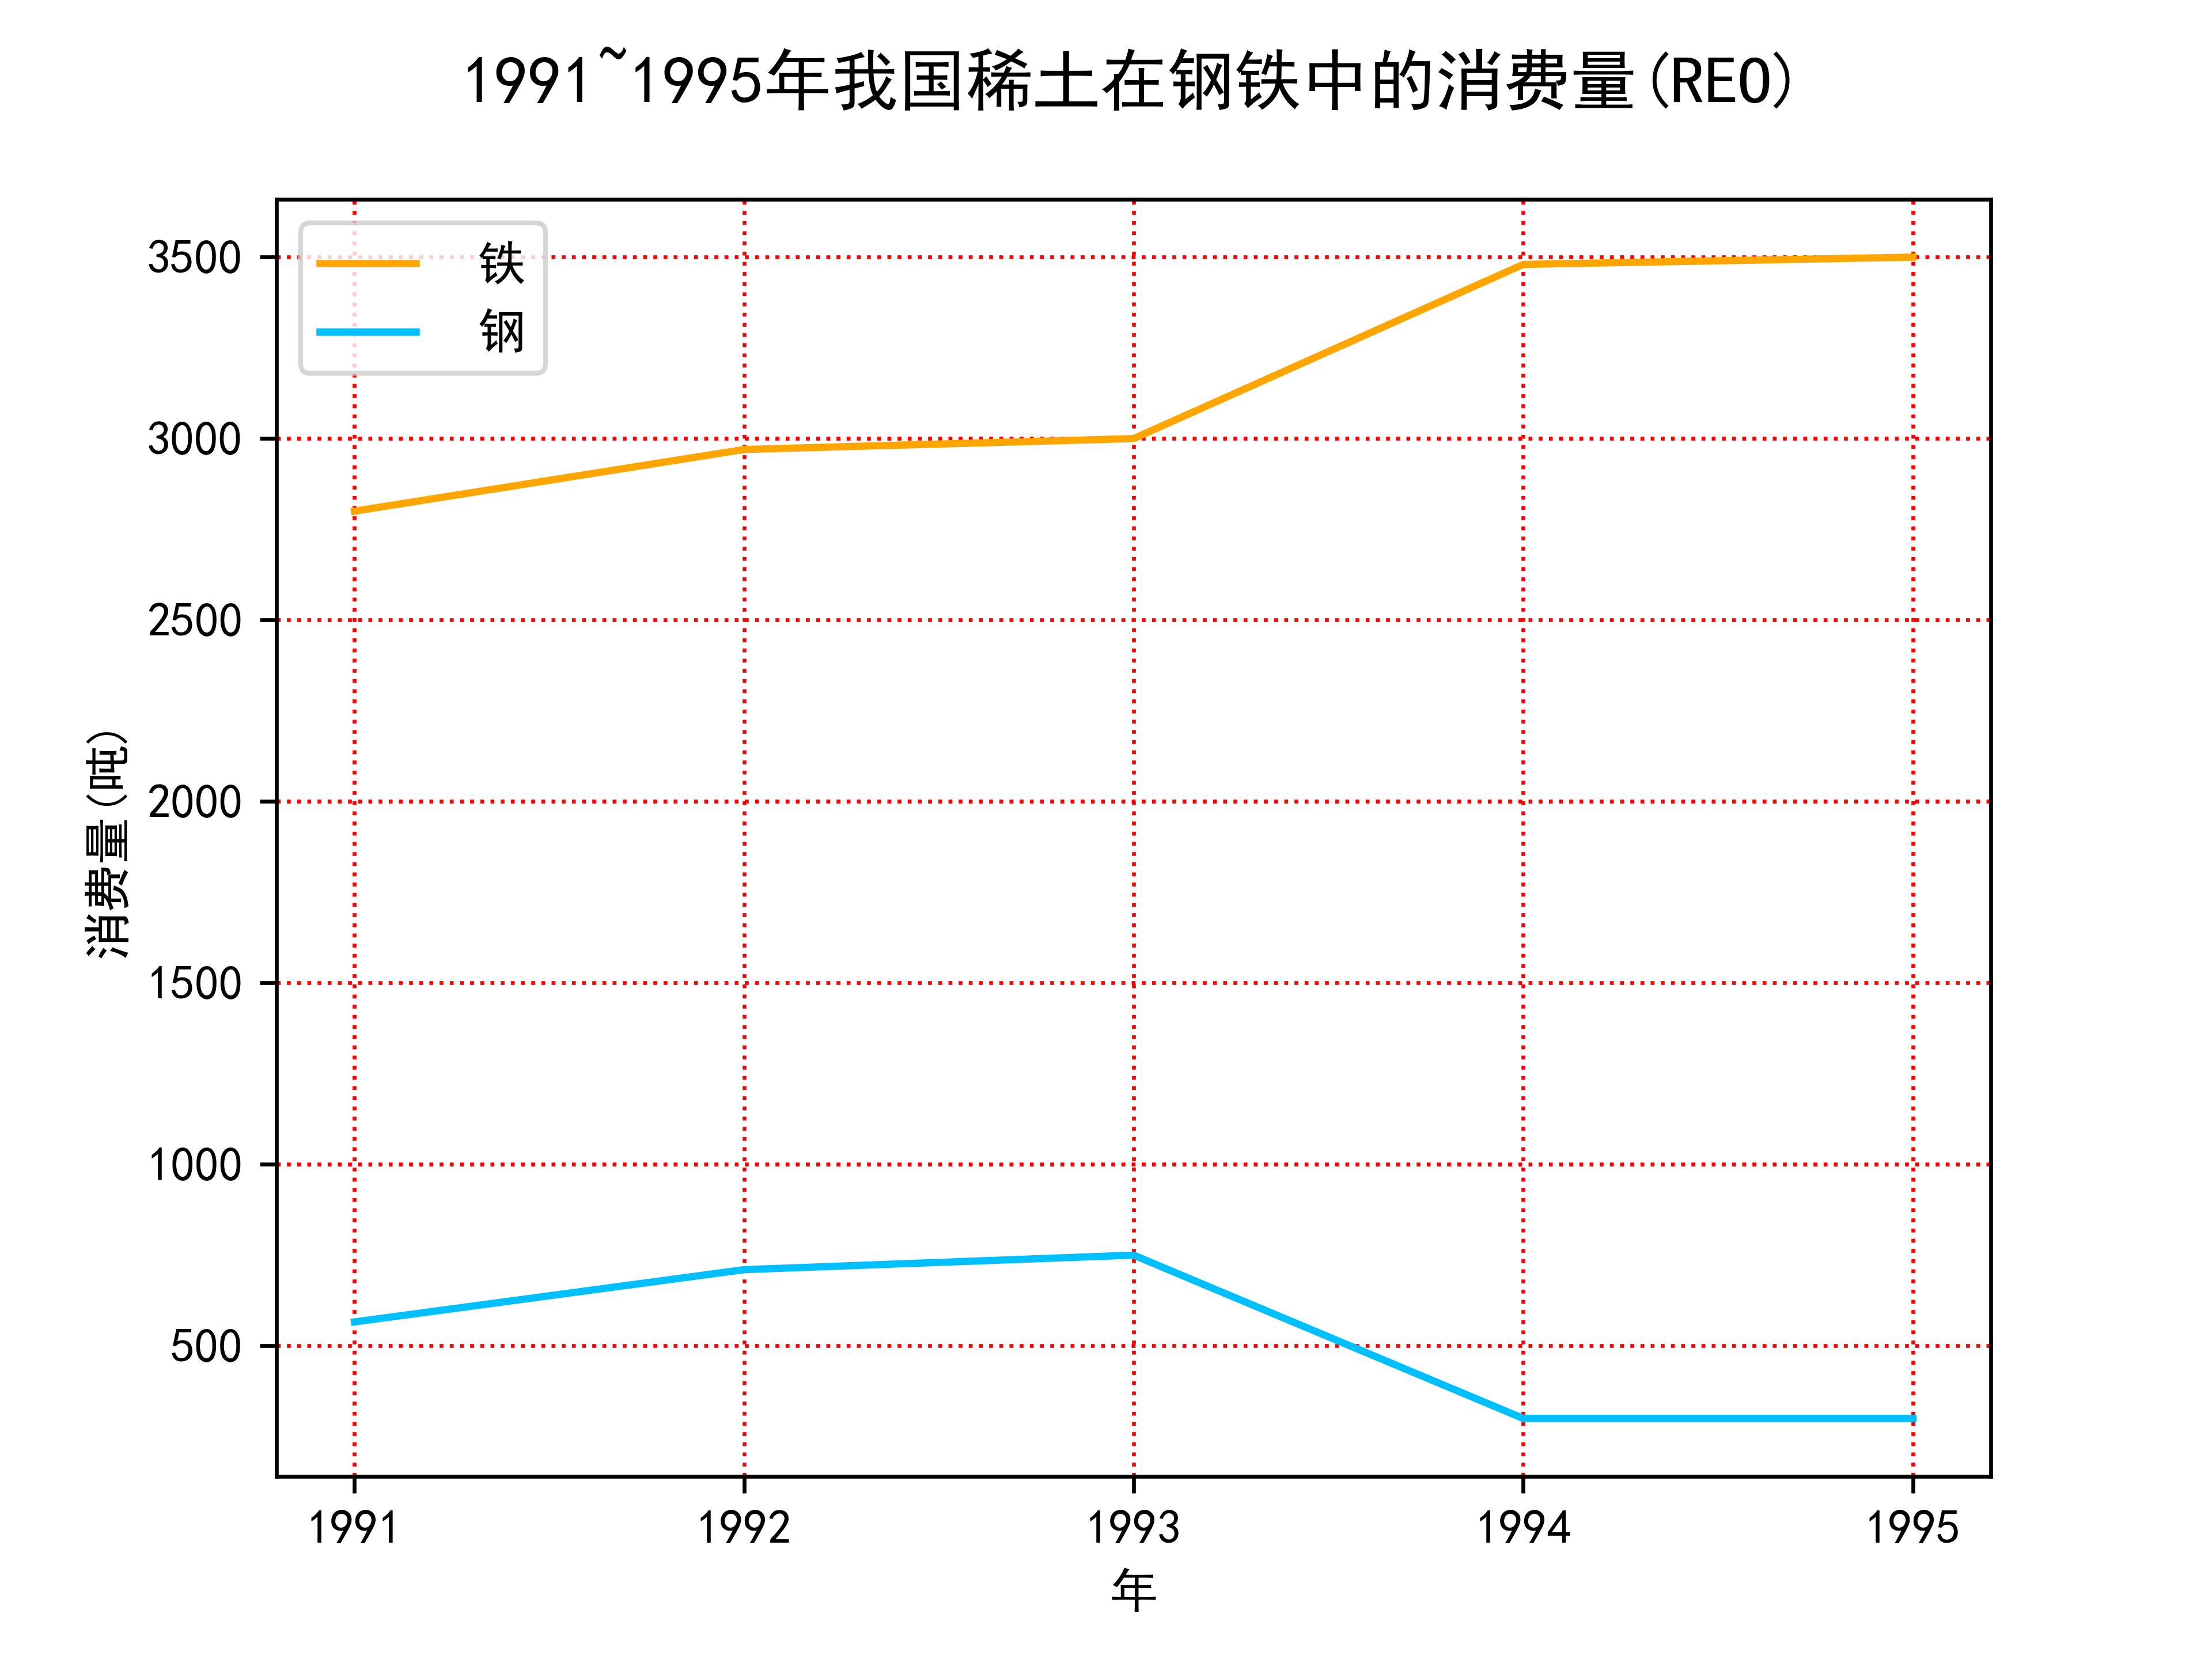
\includegraphics[width = 20em]{figure3.png}
   \caption{1991\~{}1995年我国稀土在钢铁中的消费量(REO)\cite{RN3}}
 \end{figure}

\begin{figure*}[h]
  \centering
  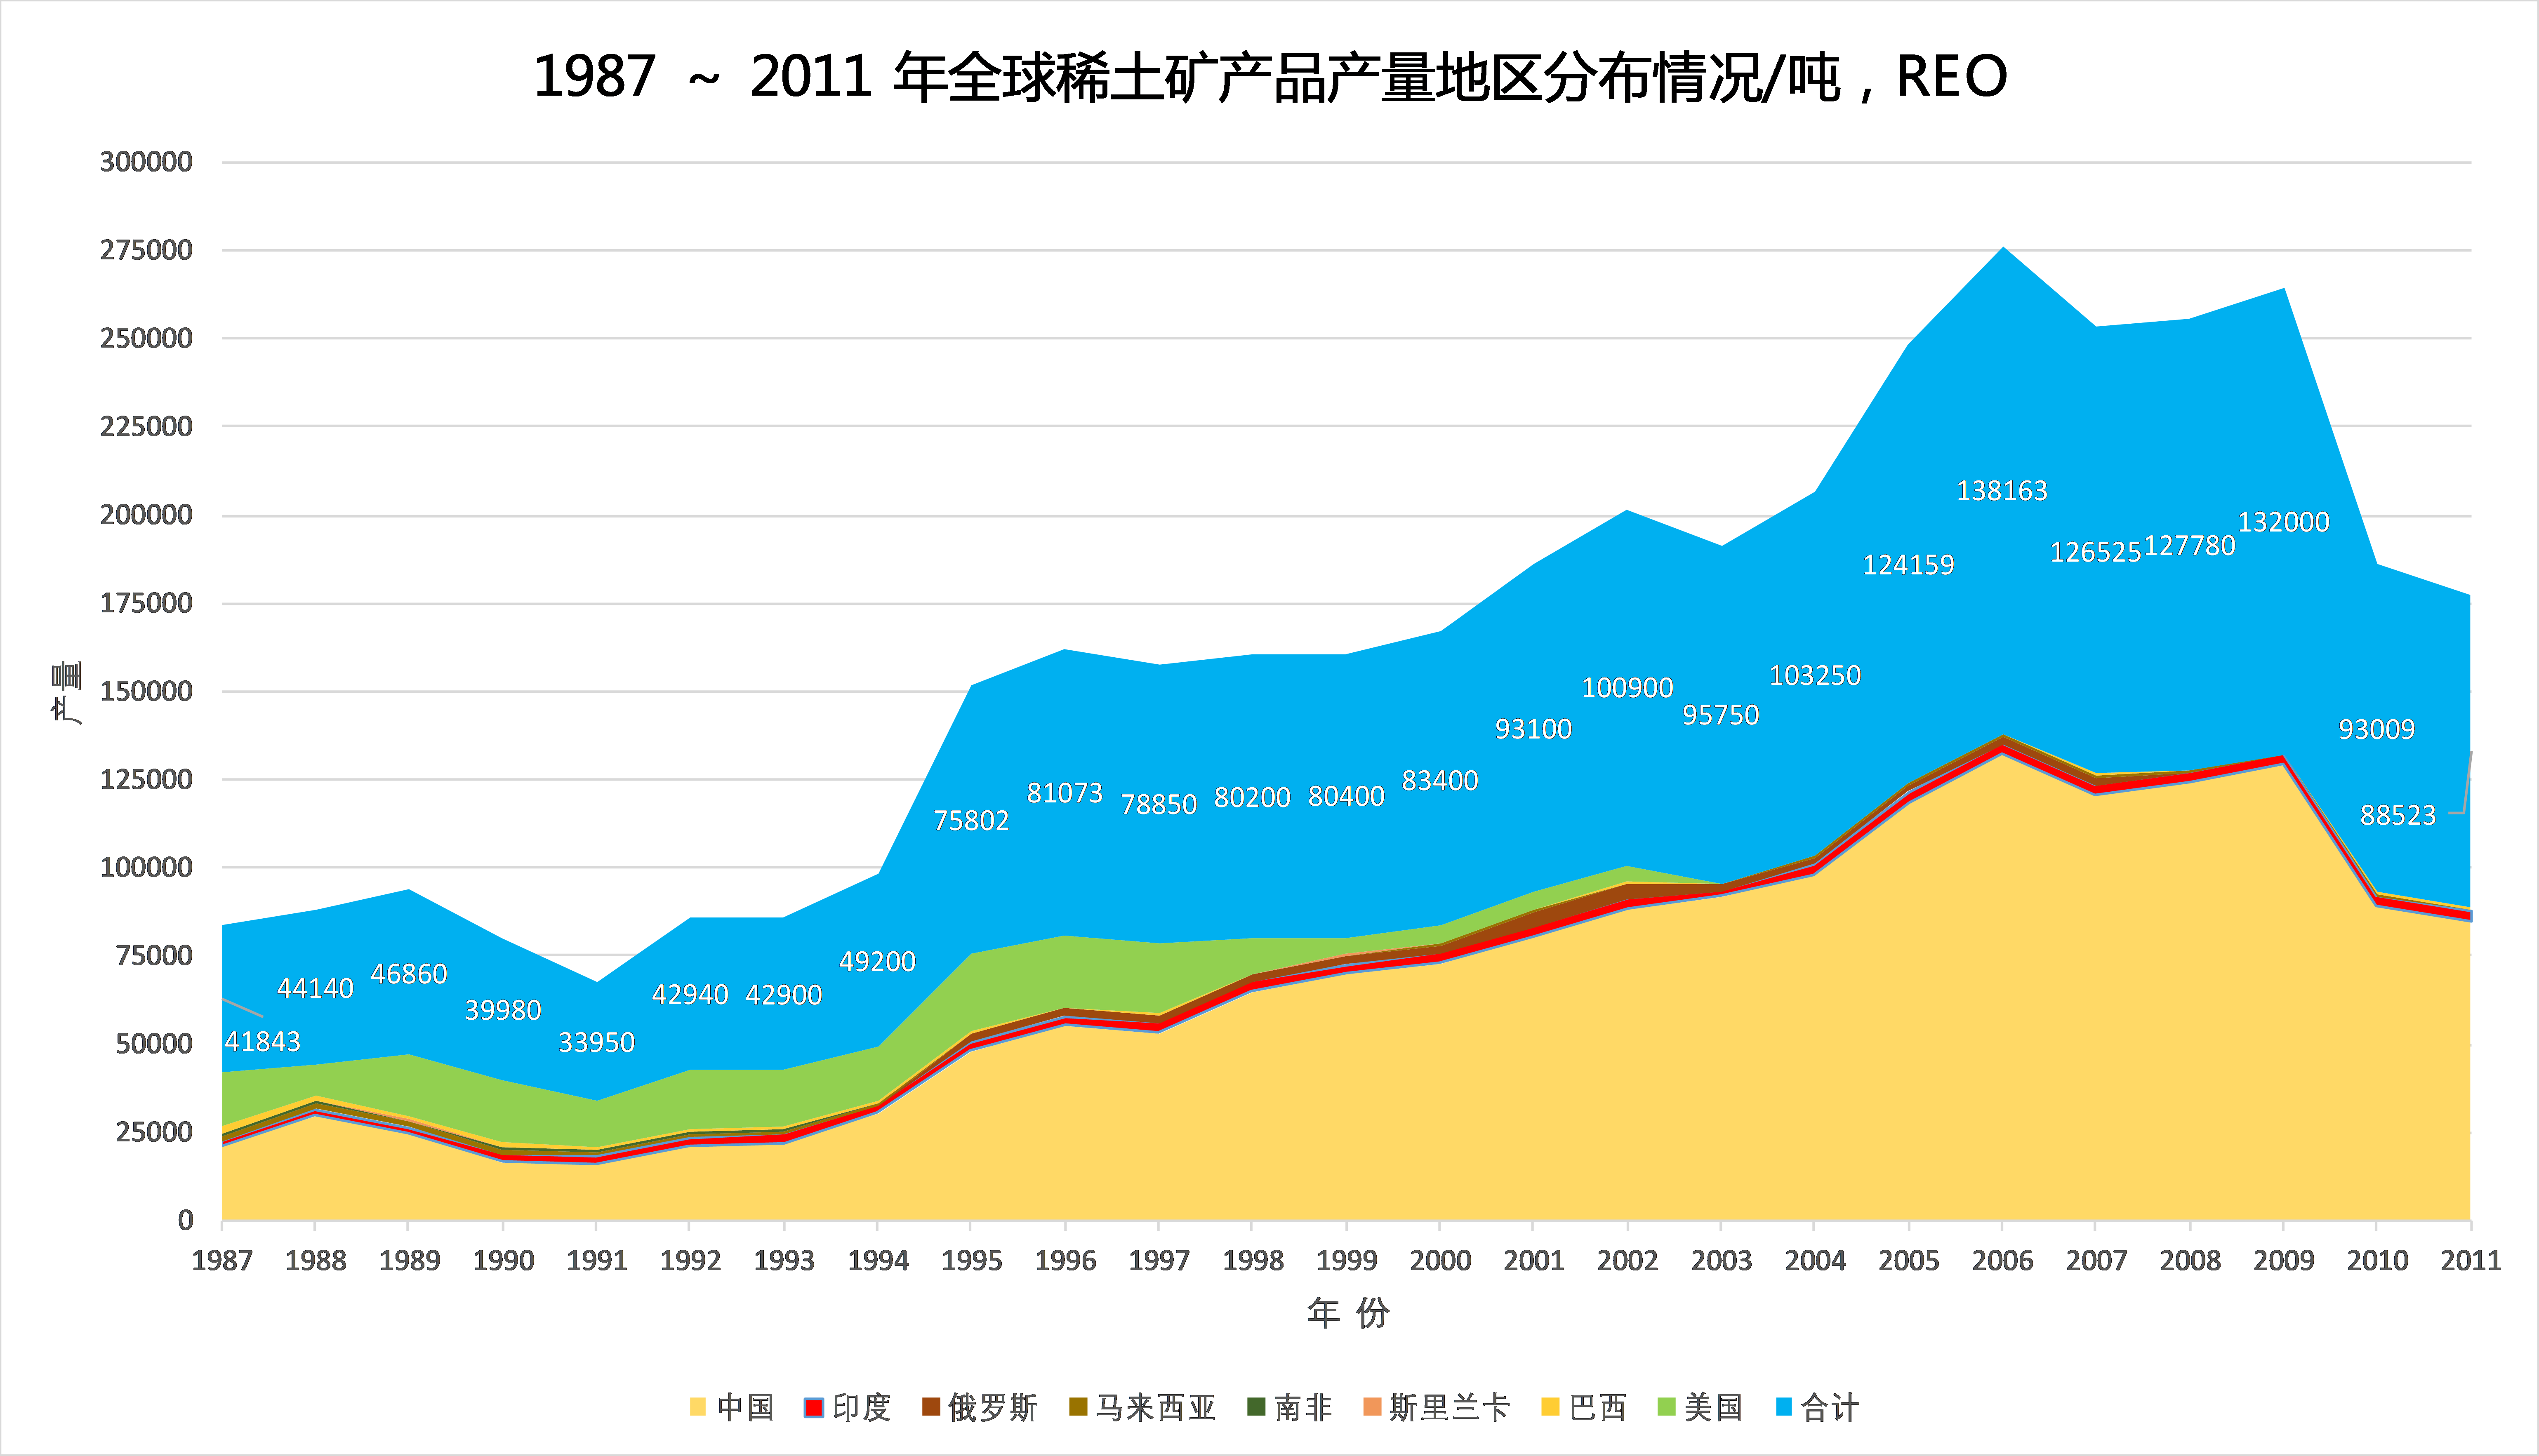
\includegraphics[width = 40em]{figure5.png}
  \caption{1987~2011 年全球稀土矿产品产量地区分布情况/吨\cite{RN6}}
\end{figure*}

在钢中的作用主要是脱硫、脱氧、细化晶粒、去除杂质等作用,从而改善钢的各项力学性能。由于稀土金属有着很高的化学活性和较大的原子半径,将其应用在有色金属及合金中能起到改善合金的作用。我国在有色金属中应用稀土起步较晚,但是该领域的需求逐年增长尤其是稀土铝合金和稀土镁合金,一直受到国家是重视。稀土变形镁合金的加工经过挤压、锻造、轧制等工艺生产出变形产品具有更高的强度、更好的延展性和更多样化的力学性能, 可以满足不同结构件的需求, 因此, 作为结构材料的稀土镁合金系列材料,适合开发变形合金产品, 生产高质量的板、棒、管、型等产品是其未来更长远的发展趋势\cite{RN52}

\subsection{石油化工领域}
目前,稀土在这一领域主要的用途是石油的催化裂化,年消费稀土约1万吨,此外还有数百吨稀土用于各种涂料与颜料等领域。自从1962年,美孚石油公司研究发现,稀土可加速石油大分子的裂化进程,稀土不仅可增加催化剂的活性,保持催化剂的热稳定性,还可增加设备的原油处理量,提高汽油产出率,降低炼油成本,于是稀土在石油的催化和裂化中便迅速展开,到1983年,美国在该领域消费的稀土量已经增加到12700吨REO,占稀土总消费量( 19600吨REO )的65$\%$ 。\cite{RN2}

另一方面,在石油需求量高涨,但是能源紧张的背景下,天然气渐渐在人们眼前变得重要了起来,相比于用贵金属来作为天然气的燃烧催化剂,使用稀土做催化剂,催化剂的活性不受高温的影响,而且在成本上也相应降低了不少。在我国华东理工大学和四川大学都对稀土作为燃烧催化剂和催化燃烧器方面做出了研究,并投入到了工业生产当中。

在高分子材料材料和合成橡胶中,稀土也作为催化剂得到了广泛应用,在以前,子午胎、高速胎等汽车轮胎多依赖国外进口,但是由于稀土的应用,使得国产新材料成功取代了进口。
\subsection{玻璃领域}
稀土在玻璃领域应用量大,花样品种繁多,稀土用于玻璃有数百年的历史, 19世纪末, 稀土开始用于玻璃作脱色澄清剂、着色剂,后来用于镜头玻璃、玻璃抛光(稀土抛光粉在本文“新材料”部分中叙述)。后来发展到用于光导纤维、防紫外线。防幅射、硬盘玻璃基片以及其它特种玻璃。现在看来,消费稀土量最多的是脱色澄清剂与镜头玻璃(不包括抛光粉)。据称2000年全球用于CRT(阴极射线管)玻璃中的稀土达1万吨。但是随着REO屏幕被LCD屏幕的取代,稀土在屏幕方面的应用也发生了改变。虽然作为屏幕的稀土被取代,但是镧玻璃在镜头方面的应用却得到了迅猛的发展,手机、数码相机、望远镜、投影仪等仪器都大量的需求镜头玻璃,据估计,现在全球一年内所需镧玻璃4000吨。\cite{RN2}

\subsection{发光材料}
由于稀土离子具有丰富的能级和4f电子跃迁特性使稀土成为一个巨大的发光宝库,为高新技术领域提供了很多性能优越的发光材料和激光材料。
\subsection{永磁材料}
稀土永磁材料的发展大致经历了三个时代,即:60年代发明的第一代水磁体SmCo3;由于Co的价格昂贵,即而开发出来了Sm2Co1型第二代永磁体,性能稳定,温度稳定性和耐腐蚀性都很好,是一种主要的水磁体;1983年美国和日本相继发明了物美价廉的Nd Fe一B第三代永磁体,其磁能积已达到432kJ/m3(5MGOe),是目前世界上磁性最强的永磁体。现在人们又在致力研究开发Sm-Fe-N系等永磁材料,有望成为第四代稀土永磁材料。\cite{RN13}目前飞速发展的电子计算机、磁电式仪表、磁悬浮系统等都已成为稀土永磁体的主要应用领域。初步统计,我国目前稀土永磁材料生产企业有200多家,总生产能力约2000吨/年。预计随着科技的发展,稀土永磁材料的用量将不断增加。
\subsection{医学领域}
稀土化合物在抗凝血方面占有特别地位,这些化合物在体内外都能降低血液的凝固,特别是静脉注射,其抗凝血作用立即产生并且能持续一天左右。\cite{RN16}

低浓度的稀土化合物水溶液具有抑菌和抗炎作用,给活体注入稀土盐能引起低血糖,因而促使人们对稀土用于治疗糖尿病的研究。同时稀土元素还具有抗癌作用,用稀土放射性同位素。1965年 Haley阐明用稀土放射性同位素可以治疗与垂体有关的肿瘤,由于垂体在肿瘤的生成中起重要作用,人们常有选择地将稀土放射性同位素作用于垂体以控制某些疾病。

\section{稀土的发展趋势分析}
中国对稀土的运用始于20 世纪60 年代中期在铸铁中的应用, 不久, 在钢中也得到应用,但是早期由于技术水平发展的落后,稀土主要作为原材料卖给国外,仅仅能获得微薄的利润。随着新兴产业的发展,稀土广泛应用于电子、能源、交通、航天、农业、医疗等13个经济领域的40多个行业,尤其对中重稀土的需求不断增加。

早期的稀土开采过程中,存在着诸多管理不善的问题,导致生态环境遭到破坏,由于生产技术落后,稀土的利用率并不高,造成资源的浪费,但是近些年国家对稀土的重视,制定出政策对稀土进行保护,取得了较好的成果。\cite{RN5}

根据美国地质勘查局统计数据显示,截止2018年底,中国稀土产量为120000吨,产量居世界第一,占世界稀土产量的71.43$\%$,近年来美国、澳大利亚稀土矿产品产量居世界前三,可见中国的稀土很有市场需求,而且需求量是稳定超其他国家的。
综上所述,从近年来世界范围内稀土的供应来源看,供应国家逐渐增加; 除中国外其他国家的供应总量将逐渐增加; 中国稀土供应比例将下降,世界稀土矿产品的供应将呈现多元化的供应格局与趋势。

通过上述分析可见,稀土产业与高新技术产业关联度密切,产品市场全球化特点突出,后续产业链的发展空间也十分广阔,是21 世纪的朝阳产业。

\begin{figure}[th]
  \centering
  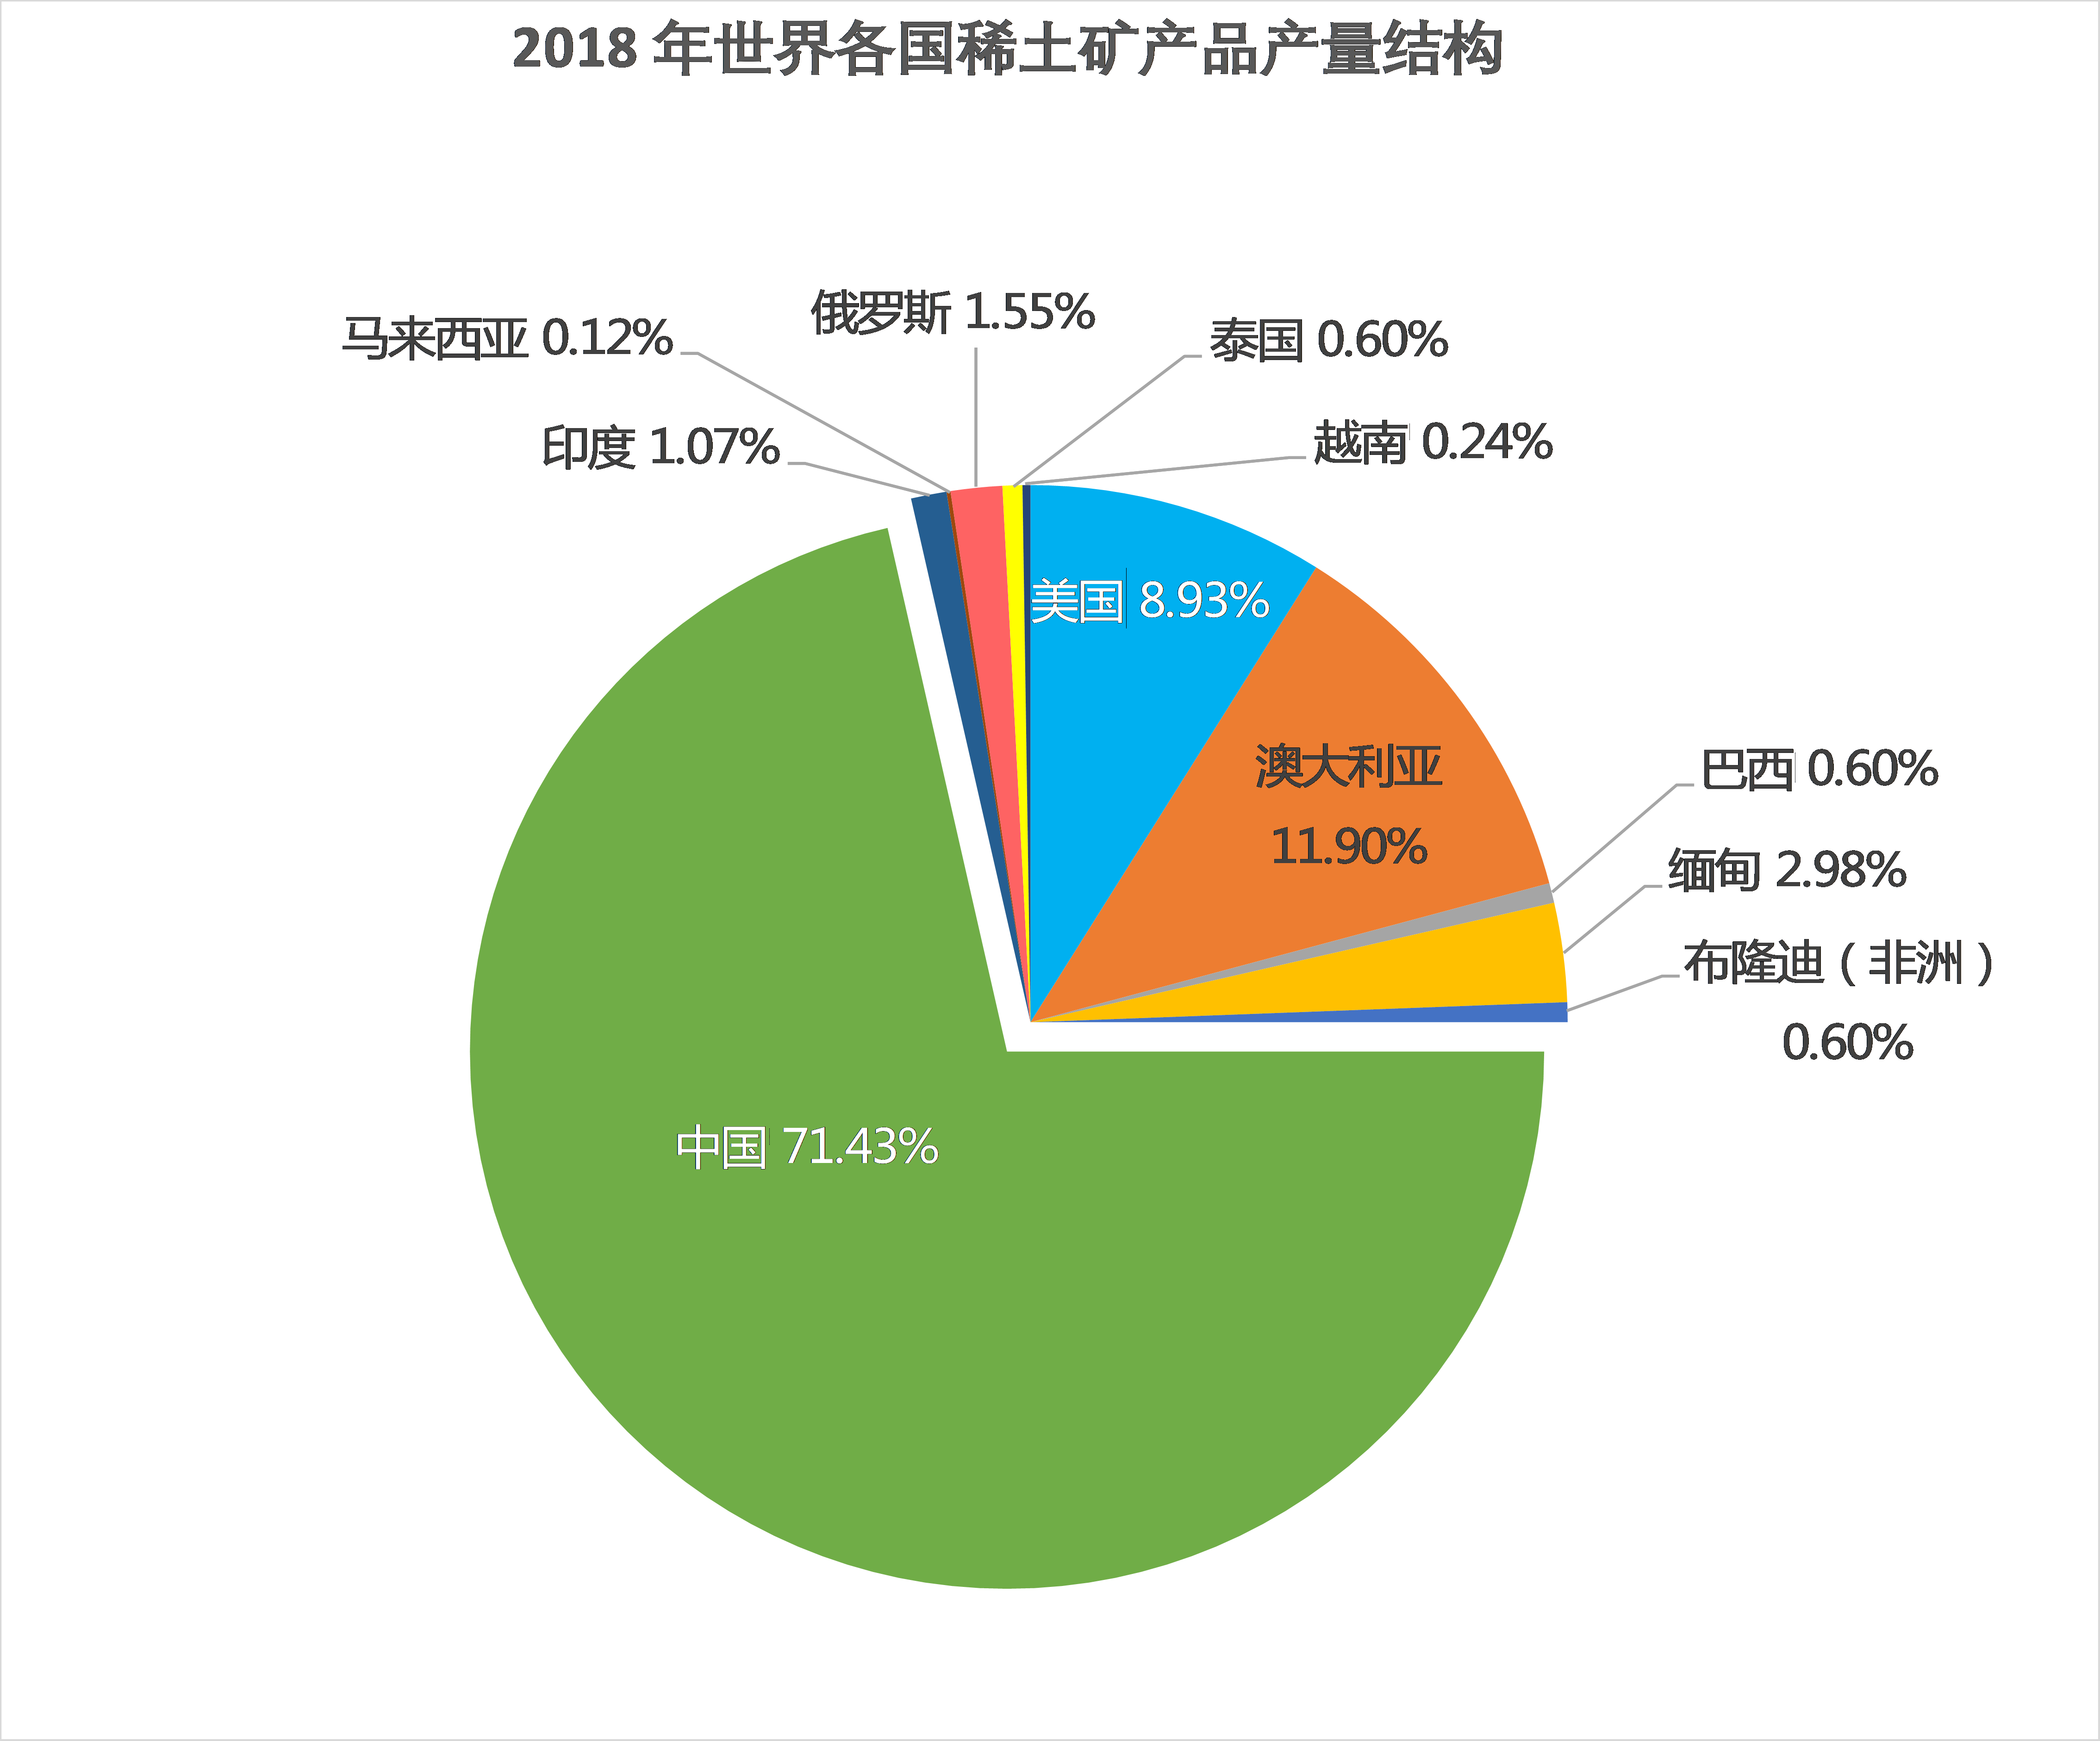
\includegraphics[width=20em]{figure1.png}
  \caption{2018 年世界各国稀土矿产品产量结构\cite{RN8}\\资料来源:U.S. Geological Survey, Mineral Commodity Summaries, February 2019}
\end{figure}

\section{结论}

我国是稀土大国,在储量和生产方面都有着相当大的优势,储量居世界第一,产量世界最多,土分布广泛,北方有山东、内蒙古,南方有四川和南方七省。在我国稀土在工业上有着非常广泛的应用,冶金领域、石油化工、玻璃都得到了很好的应用,同时稀土也作为材料被利用,稀土可以 作为发光材料、永磁材料,在合成高分子材料方面也取得了长足的进展,尤其是在永磁材料方面,随着计算机技术的发展,稀土的应用逐渐从传统工业转向了高新技术领域。在医疗方面也取得了不少的研究成果。

近些年了世界各国对稀土的需求量也在日益增加,纵观过去几十年人们对稀土的需求,始终呈现增长的趋势,人们对稀土的探索始终没有停止过,而稀土的应用也逐渐渗透到了人们生活的方方面面。随着稀土在高新技术领域的应用和在医疗方面的探索,可以看出稀土还有巨大的潜力等待人们去探索,因而而稀土在未来的发展前景是光明的。

\nocite{*}
\renewcommand\refname{\textbf{参考文献}}
\bibliography{reference}
%----------------------------------------------------------------------------------------

\end{document}
